\documentclass{article}
\usepackage[utf8]{inputenc}
\usepackage{listings}
\usepackage{color}
\usepackage[pdftex]{graphicx}
\usepackage{setspace}
\usepackage[nottoc, numbib]{tocbibind}
\usepackage[document]{ragged2e}
\usepackage{hyperref}


\begin{document}
\title{Webes alkalmazasásfejlesztés I. beadandó}
\author{Bittner Barnabás}
\maketitle
\pagebreak
\tableofcontents
\pagebreak
\section{Feladat}
\par Készítsük el egy bank ügyfelek kezelését, és az ügyfelekkel kapcsolatos tevékenységek adminisztrálását elősegítő rendszert. A webes felületen keresztül az ügyfelek érik el a bankolási funkciókat. 
 \begin{enumerate}
 	\item A főoldalon lehetőségünk van bejelentkezésre. Bejelentkezéskor meg kell adnunk a felhasználónevünket, jelszavunkat, számlaszámunkat (ha több van, akkor a legelsőt), valamint ellenőrző PIN kódunkat. Ezen felül a felhasználó választhat biztonságos üzemmódot is, ekkor minden művelet (számlatörténet lekérdezés, illetve átutalás) előtt a weblap ismét bekéri a felhasználó jelszavát. A bejelentkezést követően bármikor kijelentkezhet az ügyfél.
 	\item Sikeres bejelentkezés esetén lehetősége nyílik megtekinteni a számlái egyenlegeit (egy ügyfélhez legalább egy, de tetszőlegesen sok számla tartozhat), valamint azok történetét (átutalások, betétek, kivétek listája) egy hónapra visszamenőleg.
 	\item Lehetősége van új átutalást megadni (ha a számla nincs zárolva), ekkor ki kell tölteni az összeget, célszámla tulajdonosát, valamint számlaszámát, majd elküldhetjük az utalást, ekkor az összeg azonnal levonódik az egyenlegből (az átutalandó összeg nem lehet nagyobb a rendelkezésre álló egyenlegnél). Amennyiben a célszámla is a banknál van, akkor ott is meg kell jelennie az összegnek, mint befolyó utalás. A grafikus felületet a banki alkalmazottak használják a tranzakciók (betétek, kivételek és átutalások) kezelésére.
 	\item Az alkalmazottnak be kell jelentkeznie az alkalmazásba, ezt követően kiválaszthatja az ügyfelet, illetve annak bankszámláját.
 	\item Adott bankszámlára végezhet betétet, kivétet, illetve átutalást. Az első két esetben csak az összeget kell megadnia, míg a harmadik esetben (a webes felülethez hasonlóan) a célszámla adatait (számlaszám, tulajdonos) is. A tranzakció elküldésével az összeg azonnal levonódik/hozzáadódik az egyenleghez (átutaláskor, illetve kivételkor az összeg nem lehet nagyobb a rendelkezésre álló egyenlegnél). Amennyiben a célszámla is a banknál van, akkor ott is meg kell jelennie az összegnek, mint befolyó utalás.
 	\item Egy számla zárolható is, ekkor nem lehet semmilyen tevékenységet kezdeményezni a számlán (sem a grafikus, sem a webes felületen), amíg a zárolást fel nem oldja valamely alkalmazott. A zároláshoz a program kérjen megerősítést.
\end{enumerate}
\par Az adatbázis az alábbi adatokat tárolja (ezek még nem feltétlenül a fizikai adattáblák):
\begin{enumerate}
	\item ügyfelek (teljes név, felhasználónév, jelszó, PIN kód);
	\item alkalmazottak (teljes név, felhasználónév, jelszó);
	\item számlák (felhasználó, számlaszám, létrehozás dátuma);
	\item tranzakciók (típus, forrás számlaszám, cél számlaszám, cél tulajdonos neve, dátum, összeg).
\end{enumerate}
\section{Felhasználói dokumentáció}
A program használata rendkivül egyszerű csak egy böngészőprogramban meg kell nyitni a SmartBank weboldalát. Ha a felhasználónak még nincs fiókja regisztrálhat egyet. Regisztráció után azonnal be lehet jelentkezni, ahol a felhasználó eléri az összes saját bankszámláját, rajta az összesitett összeggel. Minden számlán le lehet kérdezni a számlatörténetet, mely után a program listázza az elmúlt havi tranzakciók listáját.  	
\subsection{Felhasználói esetek}
\begin{figure}[h]
	\caption{Use case diagram}
	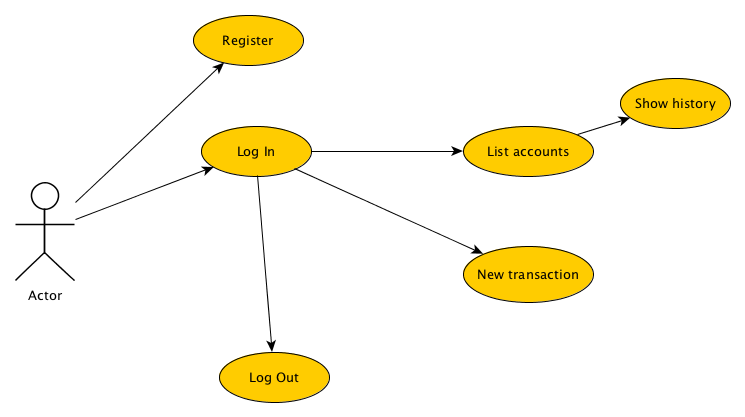
\includegraphics[scale=0.5]{usecase}
\end{figure}
\section{Fejlesztői dokumentáció}
A program alapvetően három részből áll, melyek: Core, UI, Adatbázis. Ezeket a következő szekciókban részletezem.
\subsection{Core}
A program funkcionalitásának magja, itt találhatóak az üzleti logika részei. A megvalósitás C\# WebAPI segitségével történik, a felhasználói felület HTTP hivásokkal kommunikál az üzleti logikával. A Core alapvetően a Domain Driven Design architectúrában készült, hexagonális architektúrát követve.
\begin{figure}[h]
	\caption{Core Class Diagram}
	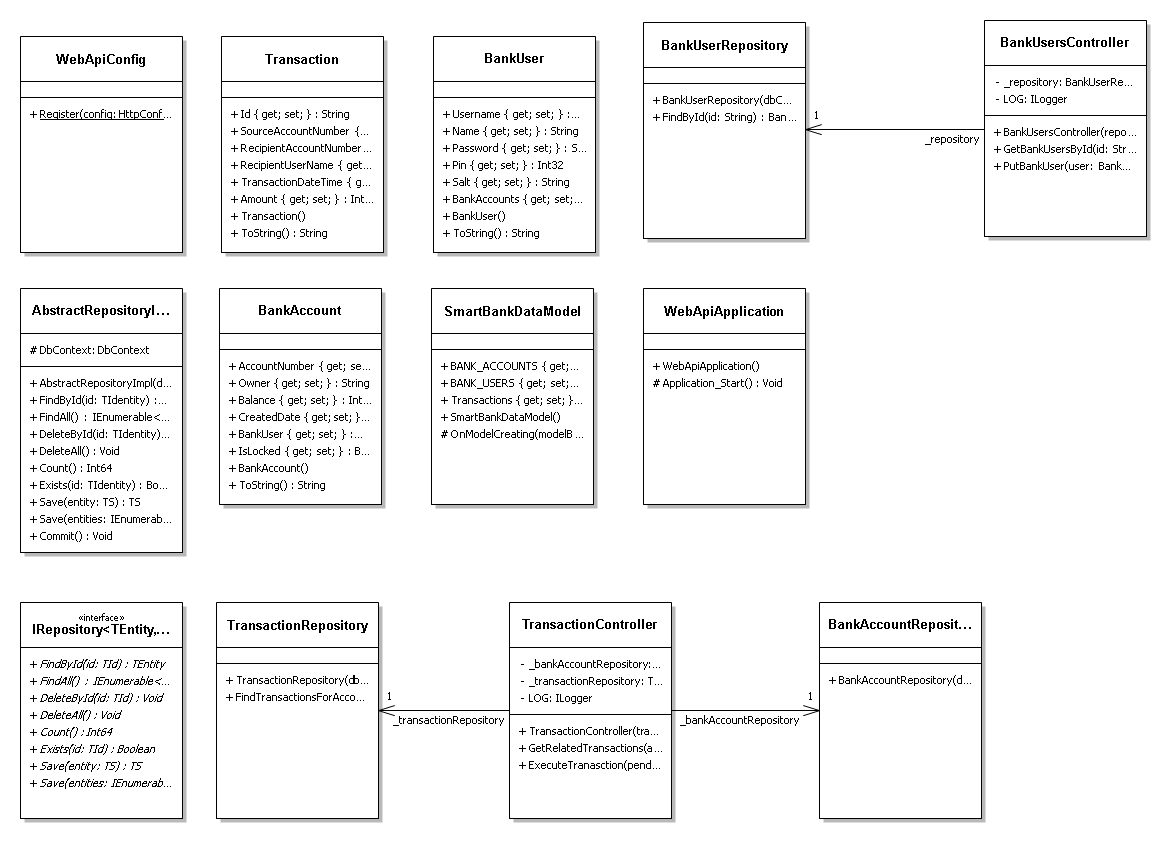
\includegraphics[scale=0.5]{SmartBankCore}
\end{figure}
\subsection{UI}
A felhasználói felület C\# ASP MVC technológiával készült el, bármilyen modern böngészőben megjelenithető. A felület HHTP hivasokkal kommunikál a core-al, amitől csak adatokat kap, amiket megfelelő módon megjelenit.
\begin{figure}[h]
	\caption{UI Class Diagram}
	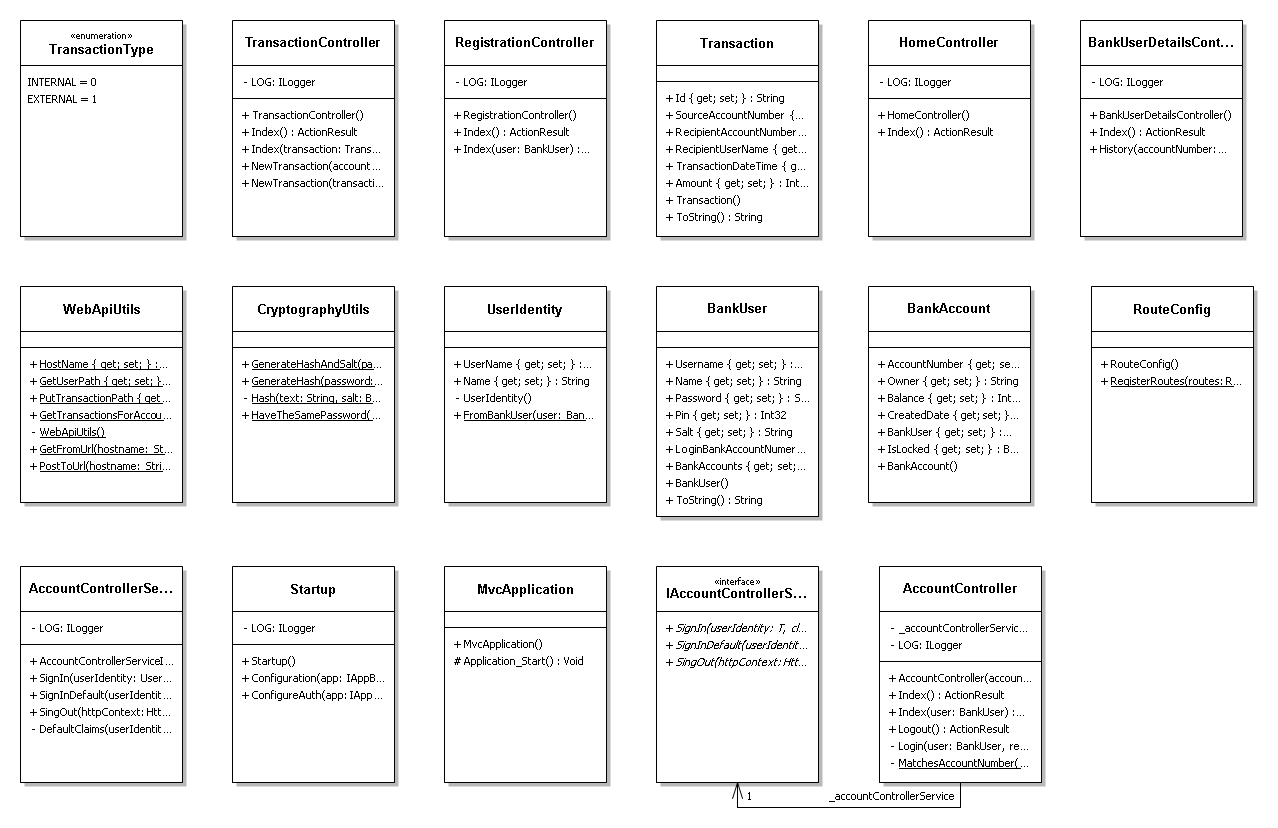
\includegraphics[scale=0.4]{SmartBankUI}
\end{figure}
\pagebreak
\subsection{Adatbázis}
A program a működéshez használt adatokat fizikai adatbázisban tárolja, melyek tartalmazzák a  regisztrált felhasználókat, azok néhány adatát. A felhasználók jelszavát enkriptálva tároljuk, esetleges adatszivárgás esetén ne lehessen (meglehetősen sok időt vegyen igénybe) a jelszavakat megszerezni. A tranzakciókat szintén az adatbázisban tároljuk, a bankszámlákkal együtt melyekhez eltároljuk a rajtuk lévő összeget. Az összeget csakis tranzakciókon keresztül lehet módositani.
\begin{figure}[h]
	\caption{Database Diagram}
	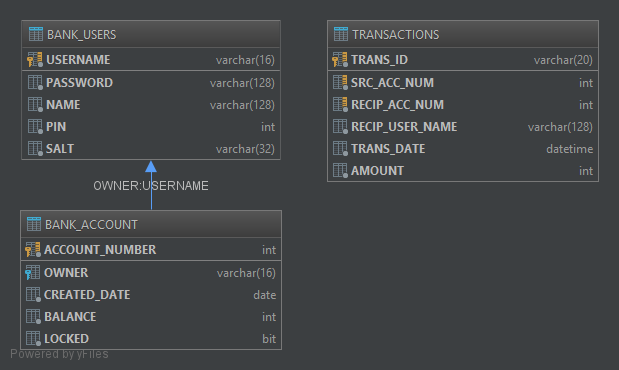
\includegraphics[scale=0.5]{DatabaseUML}
\end{figure}
\pagebreak
\section{Tesztelés}
A program helyességét Unit testekkel ellenőriztük, melyek nagyban lefedik a program által szolgált lehetőségeket. 
\end{document}
